\documentclass[openany]{book}

%% We are gonna use subfiles
\usepackage{subfiles}

%% So we can add code
\usepackage{listings}

%% Appendix package
\usepackage[toc,page]{appendix}

%% Language and font encodings
\usepackage[english]{babel}
\usepackage[utf8x]{inputenc}
\usepackage[T1]{fontenc}

% Packages for titlepage
\usepackage{columbidaeTitle}

%% Sets page size and margins
\usepackage[a4paper,top=3cm,bottom=2cm,left=3cm,right=3cm,marginparwidth=1.75cm]{geometry}

%% Useful packages
\usepackage{amsmath}
\usepackage{mathtools,xparse}
\usepackage{graphicx}
\usepackage[colorinlistoftodos]{todonotes}

\author{Tom De Groote}
\title{Machine Learning: A brief Overview}

\begin{document}
\maketitle
\tableofcontents

% Chapters
\chapter{Introduction}

%TODO schrijf introductie


\chapter{Regression}

Regression is a form of supervised machine learning with as goal to take continuous data and find the equation that best fits the data. This way you'll be able to forecast a specific value.

\section{Linear Regression}
The best fit function searched is just a linear line. See figure \ref{fig:linearregression} for an example.

\begin{figure}
\centering
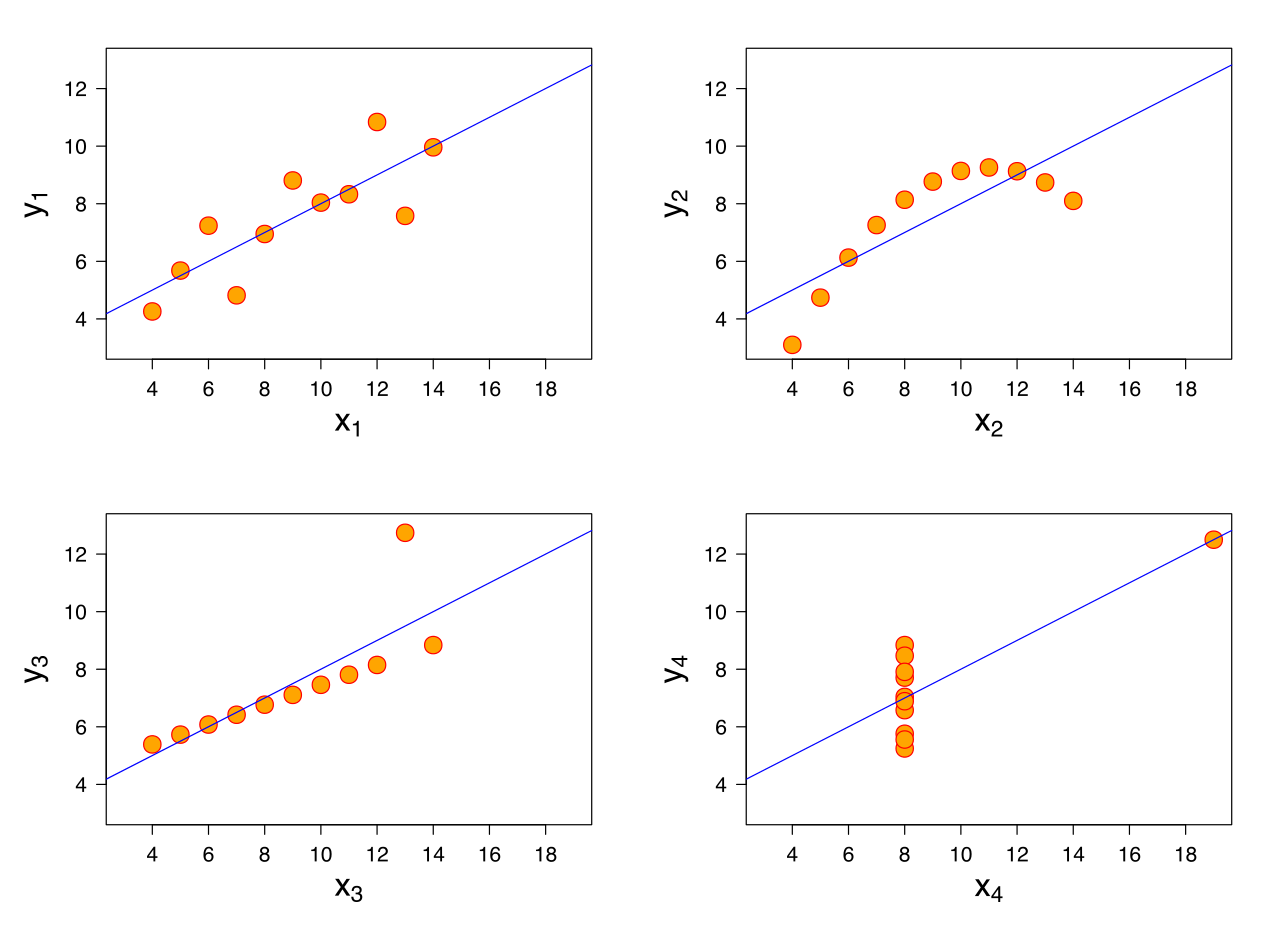
\includegraphics[width=1\textwidth]{images/linear_regression.png}
\caption{\label{fig:linearregression}Four examples of the function found by linear regression based on the given data points.}
\end{figure}

\chapter{Classification}
Classification is a form of supervised machine learning (in contrary to Clustering, see chapter \ref{chap:clustering}. It takes examples which we have identified whith classes and tries to learn a model that will predict the class of unknown examples. An example of use is to classify tumors as benign or malignant. We feed the classifier the features, such as size and shape, of known results. After the learning phase we can then use this classifier to predict if a given tumor is benign or not.

\section{K Nearest Neighbors}
K nearest neighbors is a simple but effective classification algorithm. The algorithm works by finding the k neirest neighbors of a given data point and chosing a class based on the labels of these k nearest neighbors. Basically using the majority vote of these neighbors to choose the data point's class. It is also possible to assign weight to the vote of the neighbors based on their distance.
\\
A known pitfall for the K Nearest Neighbor algorithm is that it needs to compare the data in question to all of the points from the dataset before we can know what the closest three points are. Therefor accuracy is easy to accomplish, but being fast is hard. Another way is to compare your data only to data within a certain radius. Other pitfalls include: problems with outliers and bad data.
\\
The confidence of this algorithm can be measured in two ways:
\begin{itemize}
\item Correct versus incorrect
\item Check the average vote confidence
\end{itemize}

\subsection{Code examples}
Two code approaches have been made. The first approach uses the \emph{sklearn} kit, the approach can be found in appendix \ref{code:knn}. The second approach shows a more basic KNN which illustrates it's fundamentals. This code can help you understand the basic building blocks of the algorithm and let you see where it's pitfalls are. The code can be found in appendix \ref{code:mknn}.

\section{Support Vector Machines}
A SVM is a binary classifier. The objective of the Support Vector Machine is to find the best splitting boundary between data. It is a maximum-margin-classifier. It deals in vector space, thus the seperation is done by using a hyperplane. The best hyperplane is the one that contains the widest margin between support vectors, and is called the decision boundary. It is generally much faster than the KNN algorithm and also more resistent for outliers and pointless data.
\\
\noindent Steps to find the decision boundary:
\begin{enumerate}
\item Find the support vectors, see figure \ref{fig:svm-support-vectors}. We find these support vectors by maximising the distance between all examples of the two classes.
\item The decision boundary runs through the middle of these support vectors, see figure \ref{fig:svm-decision-boundary}.
\end{enumerate}

As you may notice, this method will only work natively on linearly-seperable data and data with only two classes. %TODO hoe doen werken voor niet lineaire data en voor meer dan 2 klassen?
This is only a general overview of SVMs, for more information take a look at this SVM Tutorial\footnote{http://www.svm-tutorial.com/}.

%TODO verklaar x.w + b

\begin{figure}
\centering
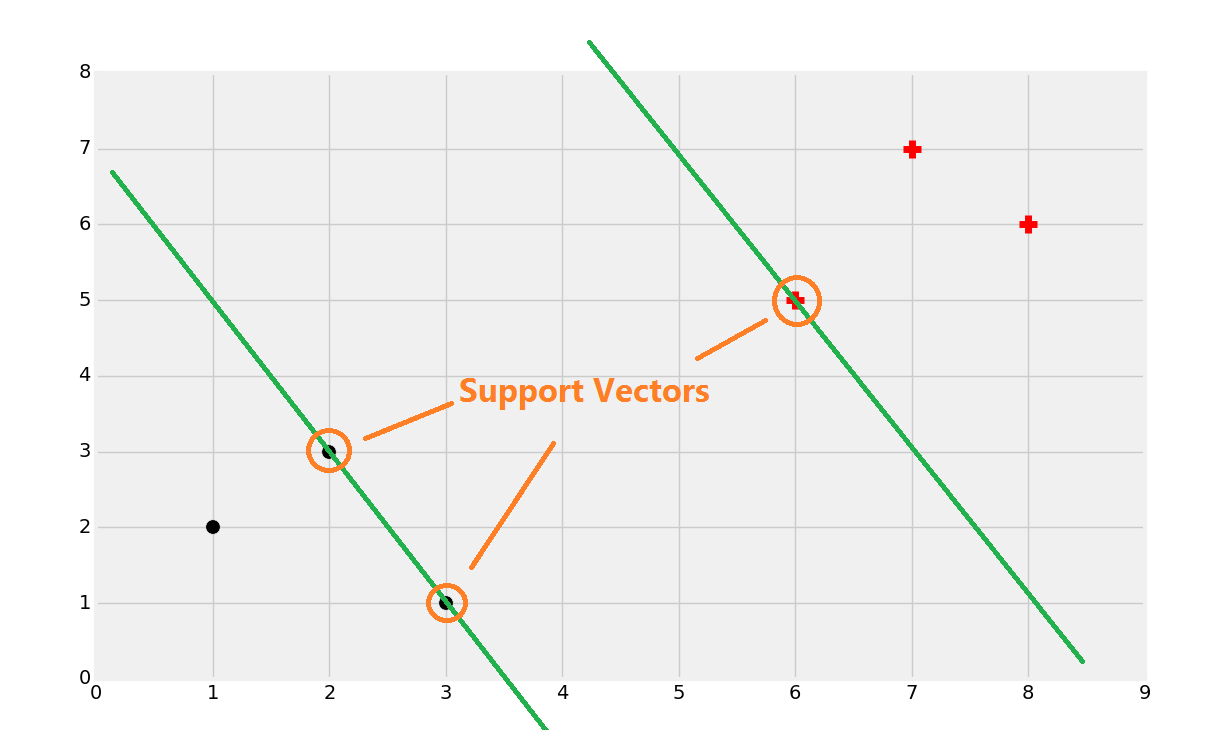
\includegraphics[width=0.8\textwidth]{images/svm-support-vectors.png}
\caption{\label{fig:svm-support-vectors} Shows the support vectors for this SVM classification problem.}
\end{figure}

\begin{figure}
\centering
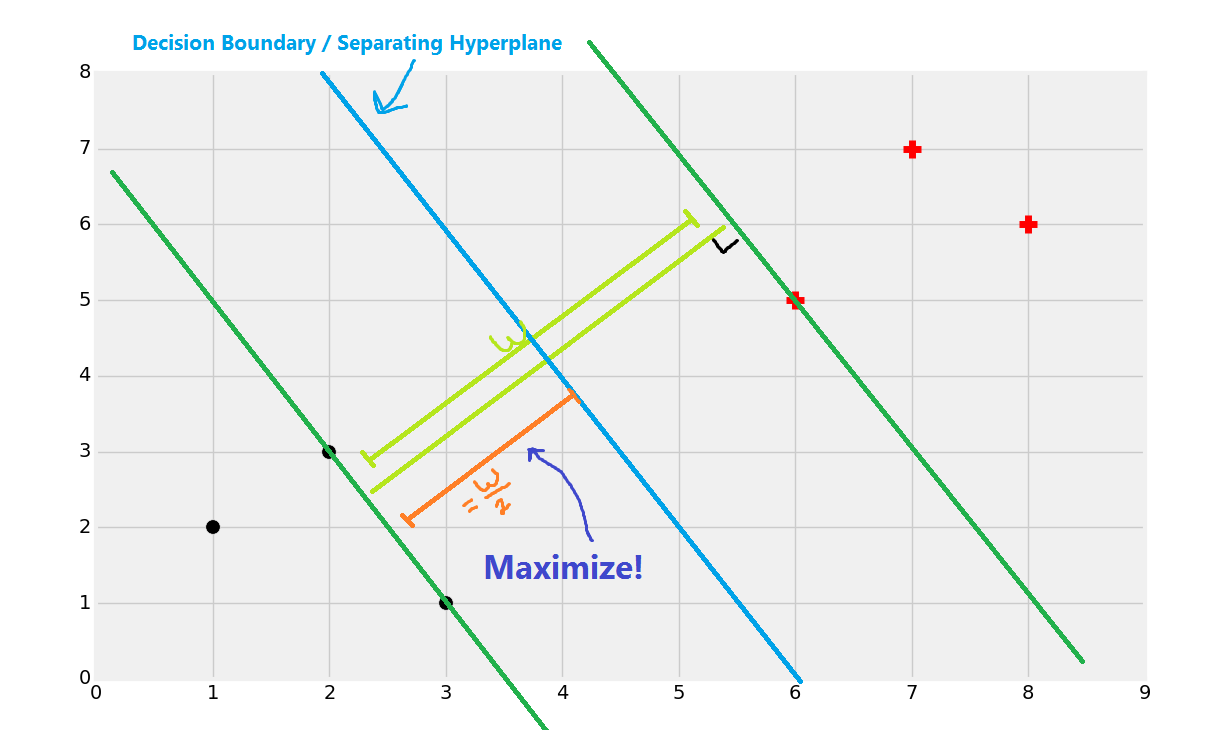
\includegraphics[width=0.8\textwidth]{images/svm-decision-boundary.png}
\caption{\label{fig:svm-decision-boundary} Shows the decision boundary for this SVM classification problem.}
\end{figure}

\subsection{Code examples}
Two code approaches have been made. The first approach uses the \emph{sklearn} kit, the approach can be found in appendix \ref{code:svm} and is very similar to appendix \ref{code:knn}. The second approach shows a more basic KNN which illustrates it's fundamentals. This code can help you understand the basic building blocks of the algorithm and let you see where it's pitfalls are. The code can be found in appendix \ref{code:msvm}.

\subsection{Support Vector Machine Regression}
It is possible to use SVMs to learn linear regression lines, as shown in our code example \ref{code:manualregression}. It tries to classify the examples by seperating them lineairly. This is done by maximising the distance between the seperating plane and the closest example of both classes, as shown in figure \ref{fig:svm}.

\begin{figure}
\centering
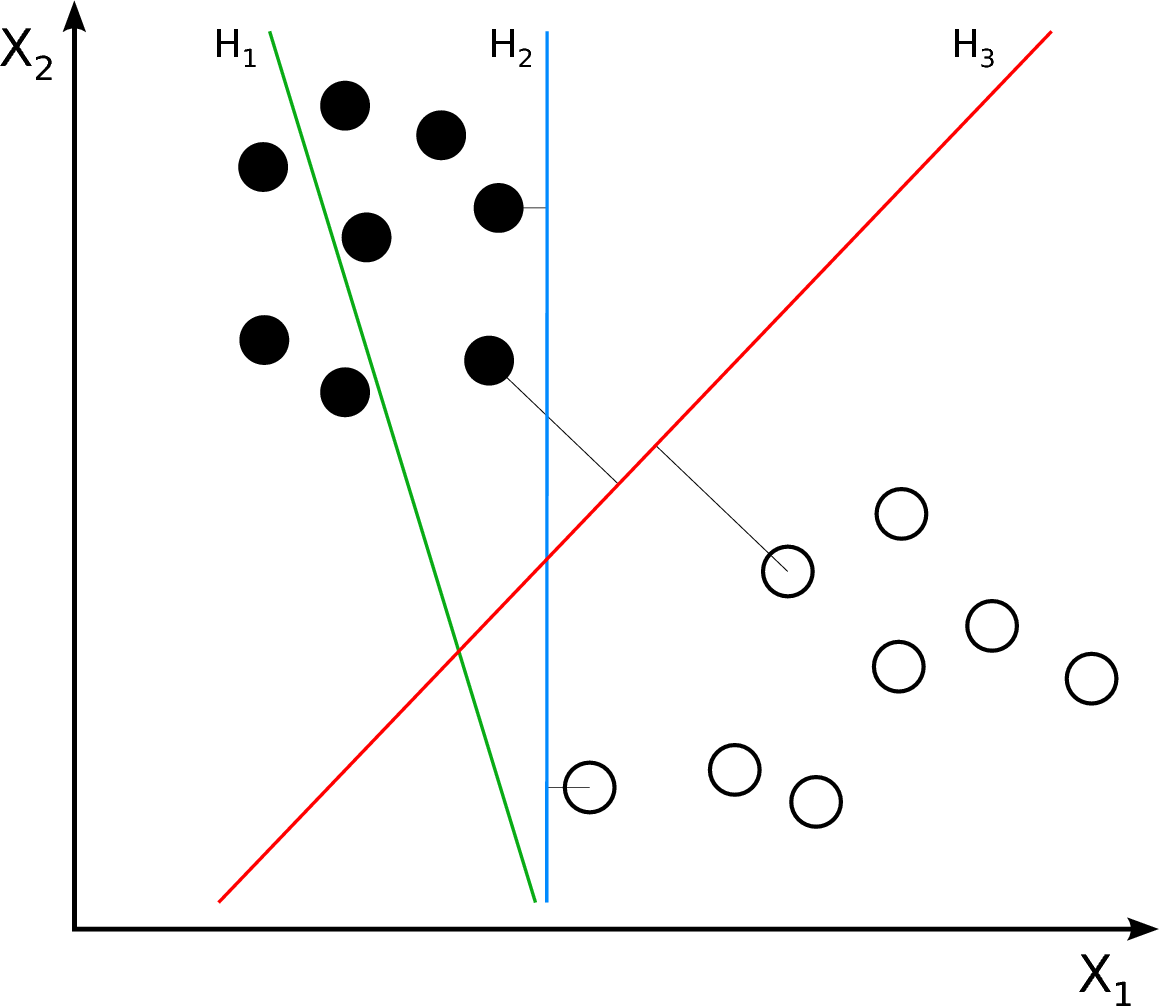
\includegraphics[width=0.4\textwidth]{images/svm.png}
\caption{\label{fig:svm} Shows three seperation planes, H1 is not a good seperating plane, H2 and H3 are acceptable.}
\end{figure}

\chapter{Clustering}\label{chap:clustering}

Clustering is a form of unsupervised learning and comes in two major forms: Flat and Hierarchical. With both forms the machine is tasked with receiving a dataset that is just featuresets, and then the machine searches for groups and assigns classes on its own. With Flat clustering the scientist tells the machine how many classes/clusters to fine. With Hierarchical clustering, the machine figures out the groups and how many. 
\\\\
The objective is to find relationships and meaninig in data. It can be used in a semi-supervised context, where the scientists use the results from clustiring for further classification or it can be used on truly unknown data, in an attempt to find some structure. Clustering can also be used for typical classificaton, you just don't need to actually feed it what the classifications are beforehand.

\section{K-Means}
K-Means tries to cluster a given dataset into K clusters. Since you have to give it the number of required clusters, it is a flat clustering algorithim. It works as follows:
\begin{enumerate}
\item Take the entire dataset, and set, randomly, K number of centroids.
\item Calculate the distance of every featureset to the centroids, and classify based on the nearest centroid.
\item Now take the mean of all groups, set these as the K centroids and repeat untill optimised. Optimisation is often measured as movement of the centroid.
\end{enumerate}

\subsection{Code examples}
Three code approaches have been made. The first approach uses the \emph{sklearn} kit's K-Means classifier to classify a simple example, the approach can be found in appendix \ref{code:kmeans}. The second approach also uses the \emph{sklearn} kit's K-Means classifier but this time to classify nonnumerical data, this approach can be found in appendix \ref{code:nonnumerical-kmeans}. The third and final approach shows a more basic K-Means classifier which illustrates it's fundamentals. This code can help you understand the basic building blocks of the K-Means classifier.  This code can be found in appendix \ref{code:manual-kmeans}.

\section{Mean Shift}
Mean Shift is very similar to the K-Means algorithm but you do not need to give it the number of clusters in advance, therefor it is a hierarchical clustering algorithm. The Mean Shift algorithm thus follows the following steps:

\begin{enumerate}
\item Make all datapoints centroids
\item Take mean of all featuresets within a centroid's radius, setting this mean as new centroid.
\item Repeat step \#2 until convergence.
\end{enumerate}

\noindent As you may notice the downside is scalability, because we have to start from every datapoint. For finding the mean in step 2 we can use a kernel, you can either use a flat kernel (here we have every featureset with the same weigth) or a Gaussian Kernel (here weight's are assigned by proximity to the kernel's center). The radius as well can be calculated based on the data, as shown in the code-example \ref{code:manual-meanshift}.

\subsection{Code examples}
Three code approaches have been made. The first approach uses the \emph{sklearn} kit's Mean Shift classifier to classify a simple example, the approach can be found in appendix \ref{code:meanshift}. The second approach also uses the \emph{sklearn} kit's Mean Shift classifier but this time to classify nonnumerical data, this approach can be found in appendix \ref{code:nonnumerical-meanshift}. The third and final approach shows a more basic Mean Shift classifier which illustrates it's fundamentals. This code can help you understand the basic building blocks of the Mean Shift classifier.  This code can be found in appendix \ref{code:manual-meanshift}.


\chapter{General Terms}\label{chap:general_terms}

\paragraph{Confidence Score} 
A score that tells you how accurate and reliable a model is performing based on the test data.

\paragraph{Convex}
%TODO bespreek convex hull, convex optimisation, in ieder geval da ding da we gebruiken voor de python tutorial 29 moeten we wel vermelden.

\paragraph{Cross Validation} 
Is a model validation technique for assessing how the results of a statistical analysis will generalize to an independent data set. It splits the data set in test and training data.

\paragraph{Deterministic Enviroment}
The endstate of the enviroment can be determined based on the current state of the enviroments and its components.

\paragraph{Decision Boundary}
In a statistical-classification problem with two classes, a decision boundary is a hyperplane that partitions the underlying vector space into two sets, one for each class.

\paragraph{Dot Product}
Also known as \emph{scalair product} or \emph{inner product} of two vectors $\vec{A}$ and $\vec{B}$ is defined as follows: $\vec{A} \cdot \vec{B} = a_1 b_1 + a_2 b_2 + ... + a_n b_n$. Two vectors are perpindicular if their dot product equals 0. Dutch translation: \emph{inwendig product}

\paragraph{Eucledian Distance}
A way to calculate the distance on a plane between points. It uses the following formula: $\sqrt{\sum\limits_{i=1}^n (q_{i} - p_{i})^2}$. Measures the length of a line segment between points.

\paragraph{Eucledian Norm}
Measures the magnitude of a vector, which is basically the length. The equation is also the same as with Eucledian Distance, the name just tells you what space you are using.

\paragraph{Features} 
Descriptive attributes for the data.

\paragraph{Hyperplane}
A hyperplane is a subspace of one dimension less than its ambient space. If a space is 3-dimensional then its hyperplanes are the 2-dimensional planes.

\paragraph{Kernels} 
Is a kind of transformation on your data. Grossly put it simplifies your data. More specifically kernel methods use kernel functions to operate in a high-dimensional, implicit feature space without ever computing the coordinates of the data in that space, but rather by simply computing the inner products between the images of all pairs of data in the feature space. This is computationally a lot better than using the raw data. For an example see figure \ref{fig:kernelmethods}.
\begin{figure}
\centering
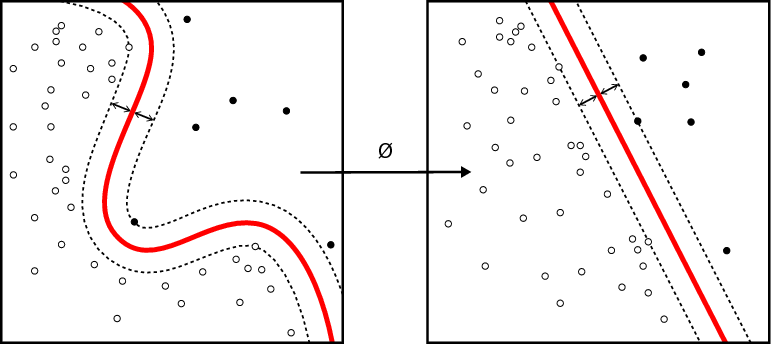
\includegraphics[width=0.4\textwidth]{images/kernelmethod.png}
\caption{\label{fig:kernelmethods} An example of simplifying the data by increasing it's dimension.}
\end{figure}

\paragraph{Labels} 
What you are trying to predict of forecast for the data.

\paragraph{Linear Algebra} 
The objective of linear algebra is to calculate relationships of points in vector space. 

\paragraph{(Maximum) Margin Classifier}
A margin classifier is a classifier which is able to give an associated distance from the decision boundary for each example. A maximum margin classifier maximises the distance between the decision boundary and all examples.

\paragraph{Object Oriented Programming}
In short OOP makes it possible to make objects with attributes, these objects can have a certain link towards eachother (subclasses and superclasses).
%TODO maak definitie OOP mooier

\paragraph{Preprocessing} 
Used to clean/scale the data before using machine learning techniques. Cleaning for example by replacing NaN data with -99 999, because it will be handled as an outlier, or by interpolating it. Scaling your features so they fall between -1 and 1 is genarally a good idea because it could make the processing faster and more accurate.

\paragraph{Machine Learning Classifier} %TODO

\paragraph{Machine Learning Model} %TODO

\paragraph{Norm} %TODO

\paragraph{Overfitting}
Figure \ref{fig:svm-overfitting} should explain overfitting perfectly.

\begin{figure}
\centering
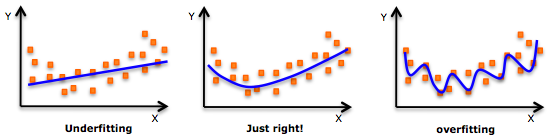
\includegraphics[width=0.8\textwidth]{images/svm-overfitting.png}
\caption{\label{fig:svm-overfitting} Shows underfitting, right fitting and overfitting.}
\end{figure}

\paragraph{Stochastic Enviroment}
The endstate of the enviroment can not be exactly determined based on the current state of the enviroment and its objects since there is randomness involved.

\paragraph{Supervised Learning} 
For om machine learning where the scientist teaches the machine by showing it features and then showing it the correct answer (lable). Once the machine is taught, the scientis will usually test the machine on some unseen data, where the scientis still knows the correct answer, but the machine doesn't.

\paragraph{R squared method}
Also known as \emph{coefficient of determination}. The squared error is the mean or sum of the distance between the solution values and the actual values. For example in Linear regression the error is the distance between the regresssion line's y values and the data's y values. The squared error is either a mean or sum of this. Squared error is used because on the one hand it normalises all errors to be positive and on the other hand it punishes outliers harder. Since the squared error is just a relative number to your dataset it has no real meaning, that's why we use the r squared method. This method uses the formula $r^2 = 1 - \frac{SE\hat{y}}{SE_{\overline{y}}}$ which is just one minus the division of the squared error of the regression line and the squared error of the mean y line. A number close to 1 means the classifier is performing well, a number close to 0 means it is performing bad. It is a good measure when trying to predict an exact future value, however if you just want to predict a general tendense it is not the best measure.

\paragraph{Support Vector}
The points closest to the maximum-margin-hyperplane, as shown in figure \ref{fig:svm-support-vectors}.

\paragraph{Threading} 
Some machine learning algorithms can be split into multiple threads, this is often indicated by the \emph{n\_ jobs} parameter in python. Others don't have this luxurary and are known as running linear.

\paragraph{Types of Data} 
With machine learning we can see our data in several groups. It is important that these groups do not overlap, since otherwise a bad representation of results could be shown.
\begin{itemize}
	\item \textbf{Training data} is the data used to train your machine learning model.
	\item \textbf{Testing data} is the data used to test your machine learning model.
	\item \textbf{Validation data} is the data used to validate your machine learning model.
\end{itemize}

\paragraph{Vector}
A vector has a \emph{magnitude} and a \emph{direction}. The \emph{magnitude} is the same as the Euclidean distance or norm. For example the $\vec{A} = [4, 3]$ has the direction 4 in dimension 1 and 2 in dimension 2, the magnitudes is $\sqrt{4^2 + 3^2} = 5$. 


 


% Code files
\begin{appendices}
\chapter{Regression}\label{code:regression}

In this appendix you can find the code for a linear regression implementation using \emph{sklearn}, as well as some examples of SVMs used for regression.
\lstinputlisting[language=Python]{/home/tom/Dropbox/Workspace/Python/PracticalML/LinearRegression/Regression.py}

\chapter{Manual Regression}\label{code:manualregression}
In this appendix you find a linear regression algorithm build from the ground up.
\lstinputlisting[language=Python]{/home/tom/Dropbox/Workspace/Python/PracticalML/LinearRegression/ManualRegression.py}

\chapter{K Nearest Neighbors}\label{code:knn}
In this appendix you can find the code for a K nearest neighbors implementation using \emph{sklearn}.
\lstinputlisting[language=Python]{/home/tom/Dropbox/Workspace/Python/PracticalML/KNearestNeighbors/KNearestNeighbors.py}

\chapter{Manual K Nearest Neighbors}\label{code:mknn}
In this appendix you find a linear K nearest neighbors build from the ground up.
\lstinputlisting[language=Python]{/home/tom/Dropbox/Workspace/Python/PracticalML/KNearestNeighbors/ManualKNearestNeighbors.py}

\chapter{Support Vector Machine}\label{code:svm}
In this appendix you can find the code for a Support Vector Machine implementation using \emph{sklearn}.
\lstinputlisting[language=Python]{/home/tom/Dropbox/Workspace/Python/PracticalML/SVM/SVM.py}

\chapter{Manual Support Vector Machine}\label{code:msvm}
In this appendix you find a Support Vector Machine build from the ground up.
\lstinputlisting[language=Python]{/home/tom/Dropbox/Workspace/Python/PracticalML/SVM/ManualSVM.py}

\chapter{K-Means}\label{code:kmeans}
In this appendix you find the use of \emph{scikit}'s K-Means classifier for simple data.
\lstinputlisting[language=Python]{/home/tom/Dropbox/Workspace/Python/PracticalML/KMeans/k-means.py}

\chapter{Nonnumerical K-Means}\label{code:nonnumerical-kmeans}
In this appendix you find the use of \emph{scikit}'s K-Means classifier for nonnumerical data.
\lstinputlisting[language=Python]{/home/tom/Dropbox/Workspace/Python/PracticalML/KMeans/nonnumerical-k-means.py}

\chapter{Manual K-Means}\label{code:manual-kmeans}
In this appendix you find the implementation of a K-Means classifier from the ground up.
\lstinputlisting[language=Python]{/home/tom/Dropbox/Workspace/Python/PracticalML/KMeans/manual-k-means.py}

\chapter{Mean Shift}\label{code:meanshift}
In this appendix you find the use of \emph{scikit}'s Mean Shift classifier for simple data.
\lstinputlisting[language=Python]{/home/tom/Dropbox/Workspace/Python/PracticalML/MeanShift/mean-shift.py}

\chapter{Nonnumerical Mean Shift}\label{code:nonnumerical-meanshift}
In this appendix you find the use of \emph{scikit}'s Mean Shift classifier for nonnumerical data.
\lstinputlisting[language=Python]{/home/tom/Dropbox/Workspace/Python/PracticalML/MeanShift/nonnumerical-mean-shift.py}

\chapter{Manual Mean Shift}\label{code:manual-meanshift}
In this appendix you find the implementation of a Mean Shift classifier from the ground up.
\lstinputlisting[language=Python]{/home/tom/Dropbox/Workspace/Python/PracticalML/MeanShift/manual-mean-shift.py}

\chapter{Create Sentiment Featureset}\label{code:create-sentiment-featureset}
In this appendix you find the implementation for creating a sentiment featureset.
\lstinputlisting[language=Python]{/home/tom/Dropbox/Workspace/Python/PracticalML/NeuralNetwork/create_sentiment_featuresets.py}

\chapter{Convolutional Neural Network}\label{code:cnn}
In this appendix you find the implementation of a convolutional neural network using TensorFlow.
\lstinputlisting[language=Python]{/home/tom/Dropbox/Workspace/Python/PracticalML/NeuralNetwork/tensorflow-cnn.py}

\chapter{Neural Network Example}\label{code:nn-example}
In this appendix you find the implementation of a simple example of a Neural Network using TensorFlow.
\lstinputlisting[language=Python]{/home/tom/Dropbox/Workspace/Python/PracticalML/NeuralNetwork/tensorflow-example.py}

\chapter{Long Short Term Menomory}\label{code:ltsm}
In this appendix you find the implementation of a LTSM using TensorFlow.
\lstinputlisting[language=Python]{/home/tom/Dropbox/Workspace/Python/PracticalML/NeuralNetwork/tensorflow-ltsm.py}

\chapter{Number Recognition using Neural Nets}\label{code:number-recognition}
In this appendix you find the implementation of a neural network using TensorFlow to implement a number recognition program.
\lstinputlisting[language=Python]{/home/tom/Dropbox/Workspace/Python/PracticalML/NeuralNetwork/tensorflow-numberrecognition.py}

\chapter{Sentiment Analyses with Neural Nets}\label{code:sentiment}
In this appendix you find the implementation of a sentiment analyses using Neural Networks from TensorFlow.
\lstinputlisting[language=Python]{/home/tom/Dropbox/Workspace/Python/PracticalML/NeuralNetwork/tensorflow-sentiment.py}

\chapter{Convolution with TFLearn}\label{code:tflearn}
In this appendix you find the implementation of a convolutional neural net using TFLearn.
\lstinputlisting[language=Python]{/home/tom/Dropbox/Workspace/Python/PracticalML/NeuralNetwork/tflearn-convolution.py}
%TODO some code falls out of the page, fix this
\end{appendices}

\end{document}